\chapter{Engineering Rationale}
This chapter reviews and justifies the choice of software used in the stack for this project.

\section{Cross-Platform Frameworks}
A long standing problem in the development of mobile applications has been that of having to maintain multiple codebases in order to increase user reach. Especially since different platforms almost always use completely different workflows and programming languages, this means having to employ multiple teams just to maintain separate codebases, leading to features being rolled out on one platform before another, or an inconsistent user experience between both platforms.

Cross-platform development seeks to solve this problem, often by creating a workflow in a given language which may then be transpiled into native platform code. While this solves the aforementioned problem, it also creates problems of its own. Cross-platform frameworks usually offer a reduced set of features compared to their native counterparts, since they effectively have to duplicate the API that the native platform exposes using different language semantics, which may not even be possible in some cases.

Despite this, cross-platform frameworks have found their niche in helping small teams of developers bring a concept to market quickly. It is for this reason that this project will use a cross-platform framework in order to bring the product to iOS in a way that is extensible for future work, especially since no feature in this app requires the complexity that native development offers. The following subsections will evaluate the current two most popular choices of cross-platform frameworks.

\subsection{Flutter}
Flutter is a recent framework released in 2017 by Google, aiming to provide a set of out-of-the-box interface elements to enable quick development of beautiful user interfaces. As of the time of writing, Flutter has full support for iOS 14, Android 11, macOS, Windows and web \cite{fluttersupportedplatforms}.

However, the primary criticism of Flutter is not only its age, but that it runs in Dart, another language made by Google. This means that not as much libraries and packages for flutter are limited, which means likely having to write much more first-hand code and less stable releases of libraries.


\subsection{React Native}
React Native was released by Facebook in 2014 and continues to be one of the most developed open source projects on Github (alongside Flutter). It builds off of the Model-View-Update architecture originally implemented by React and shares many domain-specific semantics. It runs on JavaScript, which is by a large margin the world's most popular programming language \cite{sfdevsurvey} and therefore has full access to the open-source library distribution channels that it offers. This mean stable support on well-developed and community endorsed packages that enforce a standardised implementation of many common features that developers use.

The result is a smooth cross-platform experience that offers close-to-native performance and a fully-functioning native bridge to give developers full flexibility in writing native code where necessary. The success of React Native has attracted many reputable companies to build their platforms with it, such as Walmart, UberEats, Bloomberg and Pinterest \cite{rnplatforms}.

\subsection{Comparison}
The primary cause of concern regarding framework choice in this project is which one best enables speed of development. This project is scoped, designed and executed by a single engineer. The scope proposed so far is usually the work of multiple full-time software engineering teams. The age and reduced developer community size for Flutter is therefore a deal-breaker in this case. The NPM registry for JavaScript currently boasts over 1 million packages in comparison to its Flutter equivalent, pub.dev which currently has around 21000. Developer documentation and community FAQ pages are also likely to have answers to issues on JavaScript rather than Dart, which means much more time can be spent focusing on higher level application design instead of "re-inventing the wheel".

\section{Cloud Hosting Vendors}
Based on requirements so far, the application will also require a back-end with a database for persistent storage of user data. This, along with what will potentially be the web version of the app, will require hosting on a server. This section briefly evaluates a selection of popular cloud service vendors and how their offerings are relevant to the requirements of this project.

The offering of a Cloud-service provider can be thought of as the balance of two philosophies: "bare-metal" providers, and managed solutions. Bare-metal refers to the act of simply provisioning computing resources on a machine, the specifics of which are left up to the user to implement. The state-of-the-art nowadays would be for a developer to specify a containerised environment using a tool such as Docker or Kubernetes, effectively creating an isolated "container" which contains all the environmental requirements needed to run a desired program. A bare-metal service would then simply bill the developer based on pre-defined billing criteria such as CPU runtime, memory usage and network bandwidth consumption.

\begin{figure}[h]
    \begin{center}
        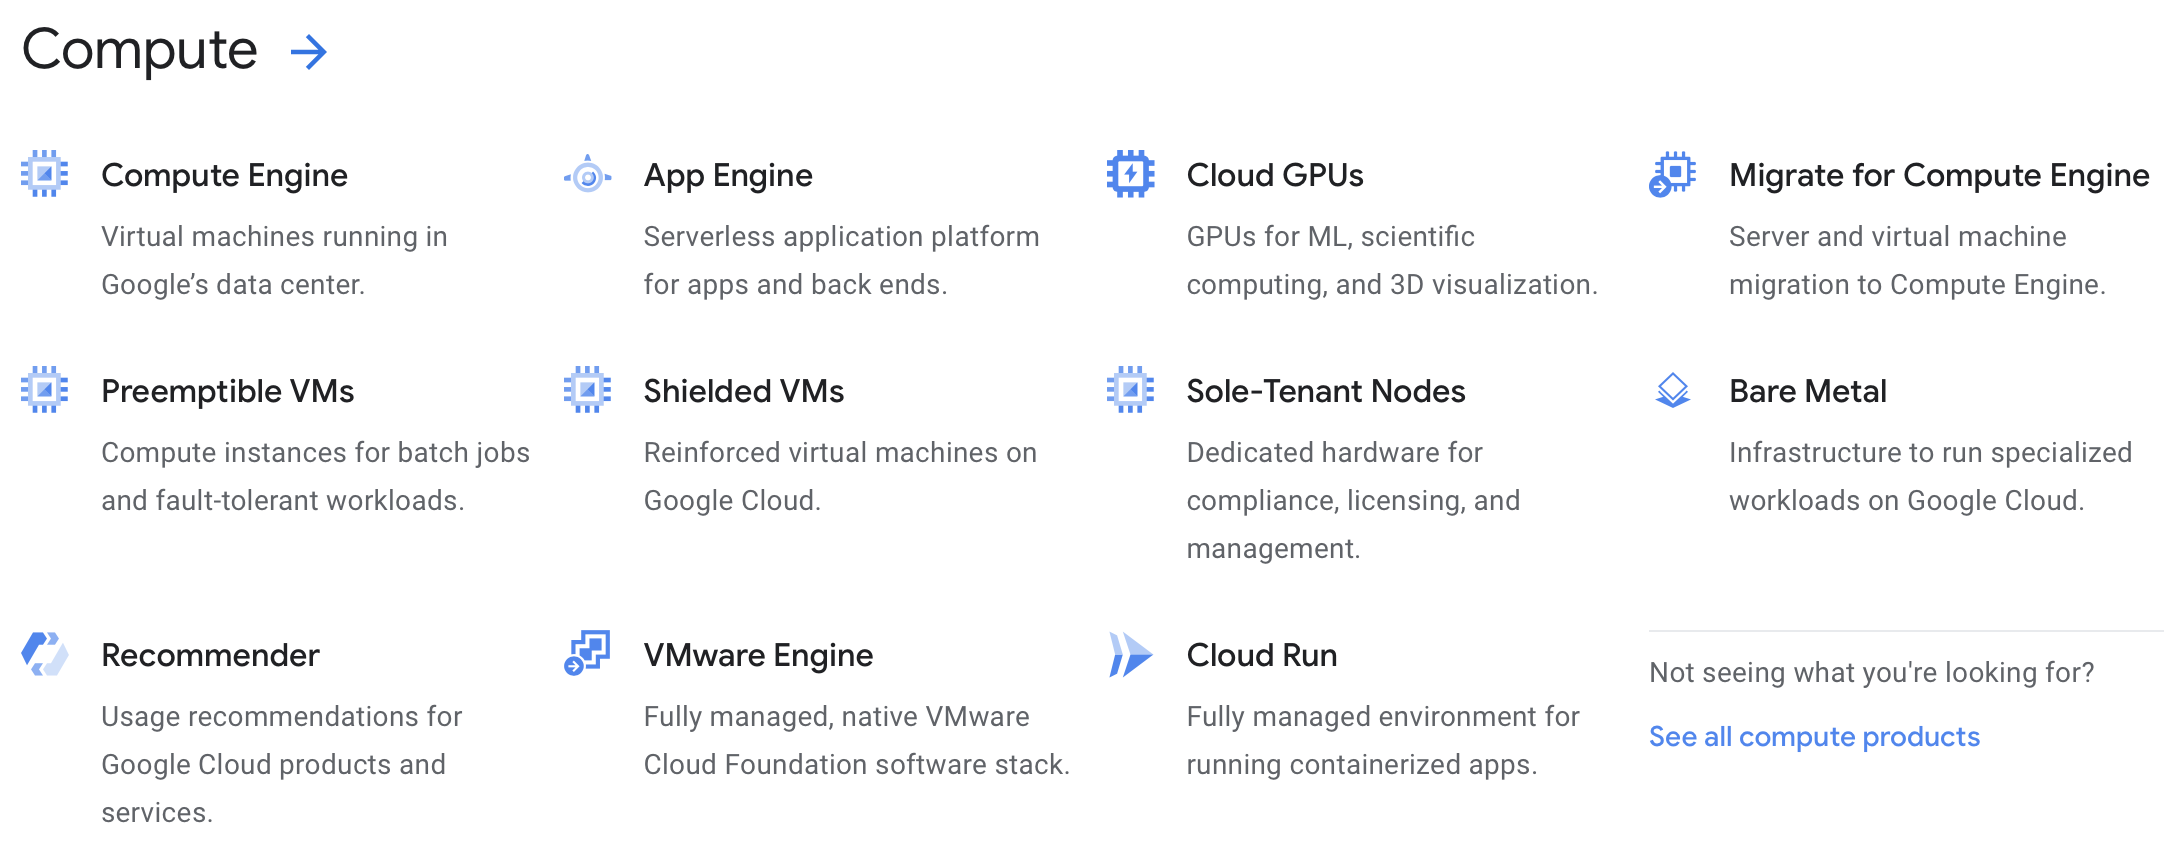
\includegraphics[scale=0.4]{images/google_cloud_compute_offerings.png}
    \end{center}
    \caption{Google Cloud compute product offerings}
    \label{gcp_compute_offerings}
\end{figure}

Managed solutions are built on top of the bare-metal philosophy. Cloud service providers may have specific offerings which deliver value to their customers in the form of pre-defined APIs which achieve a commonly desired functionality, such as user authentication. The market-leading solutions often provide a modular product selection that gives a developer a large degree of freedom to build suitable solution. One example of this is Google Cloud, which offers different degrees of control within its compute offerings, ranging from fully managed to completely bare metal.

\subsection{Firebase}
Firebase began as a startup that was later acquired by Google and now stands as one of the most popular backend-as-a-service platforms for developers looking to get small projects off of the ground. Firebase currently offers an unparalleled out-of-the-box offering for implementing safe user authentication, identity management, database and on-demand cloud compute.

\begin{figure}[h]
    \begin{center}
        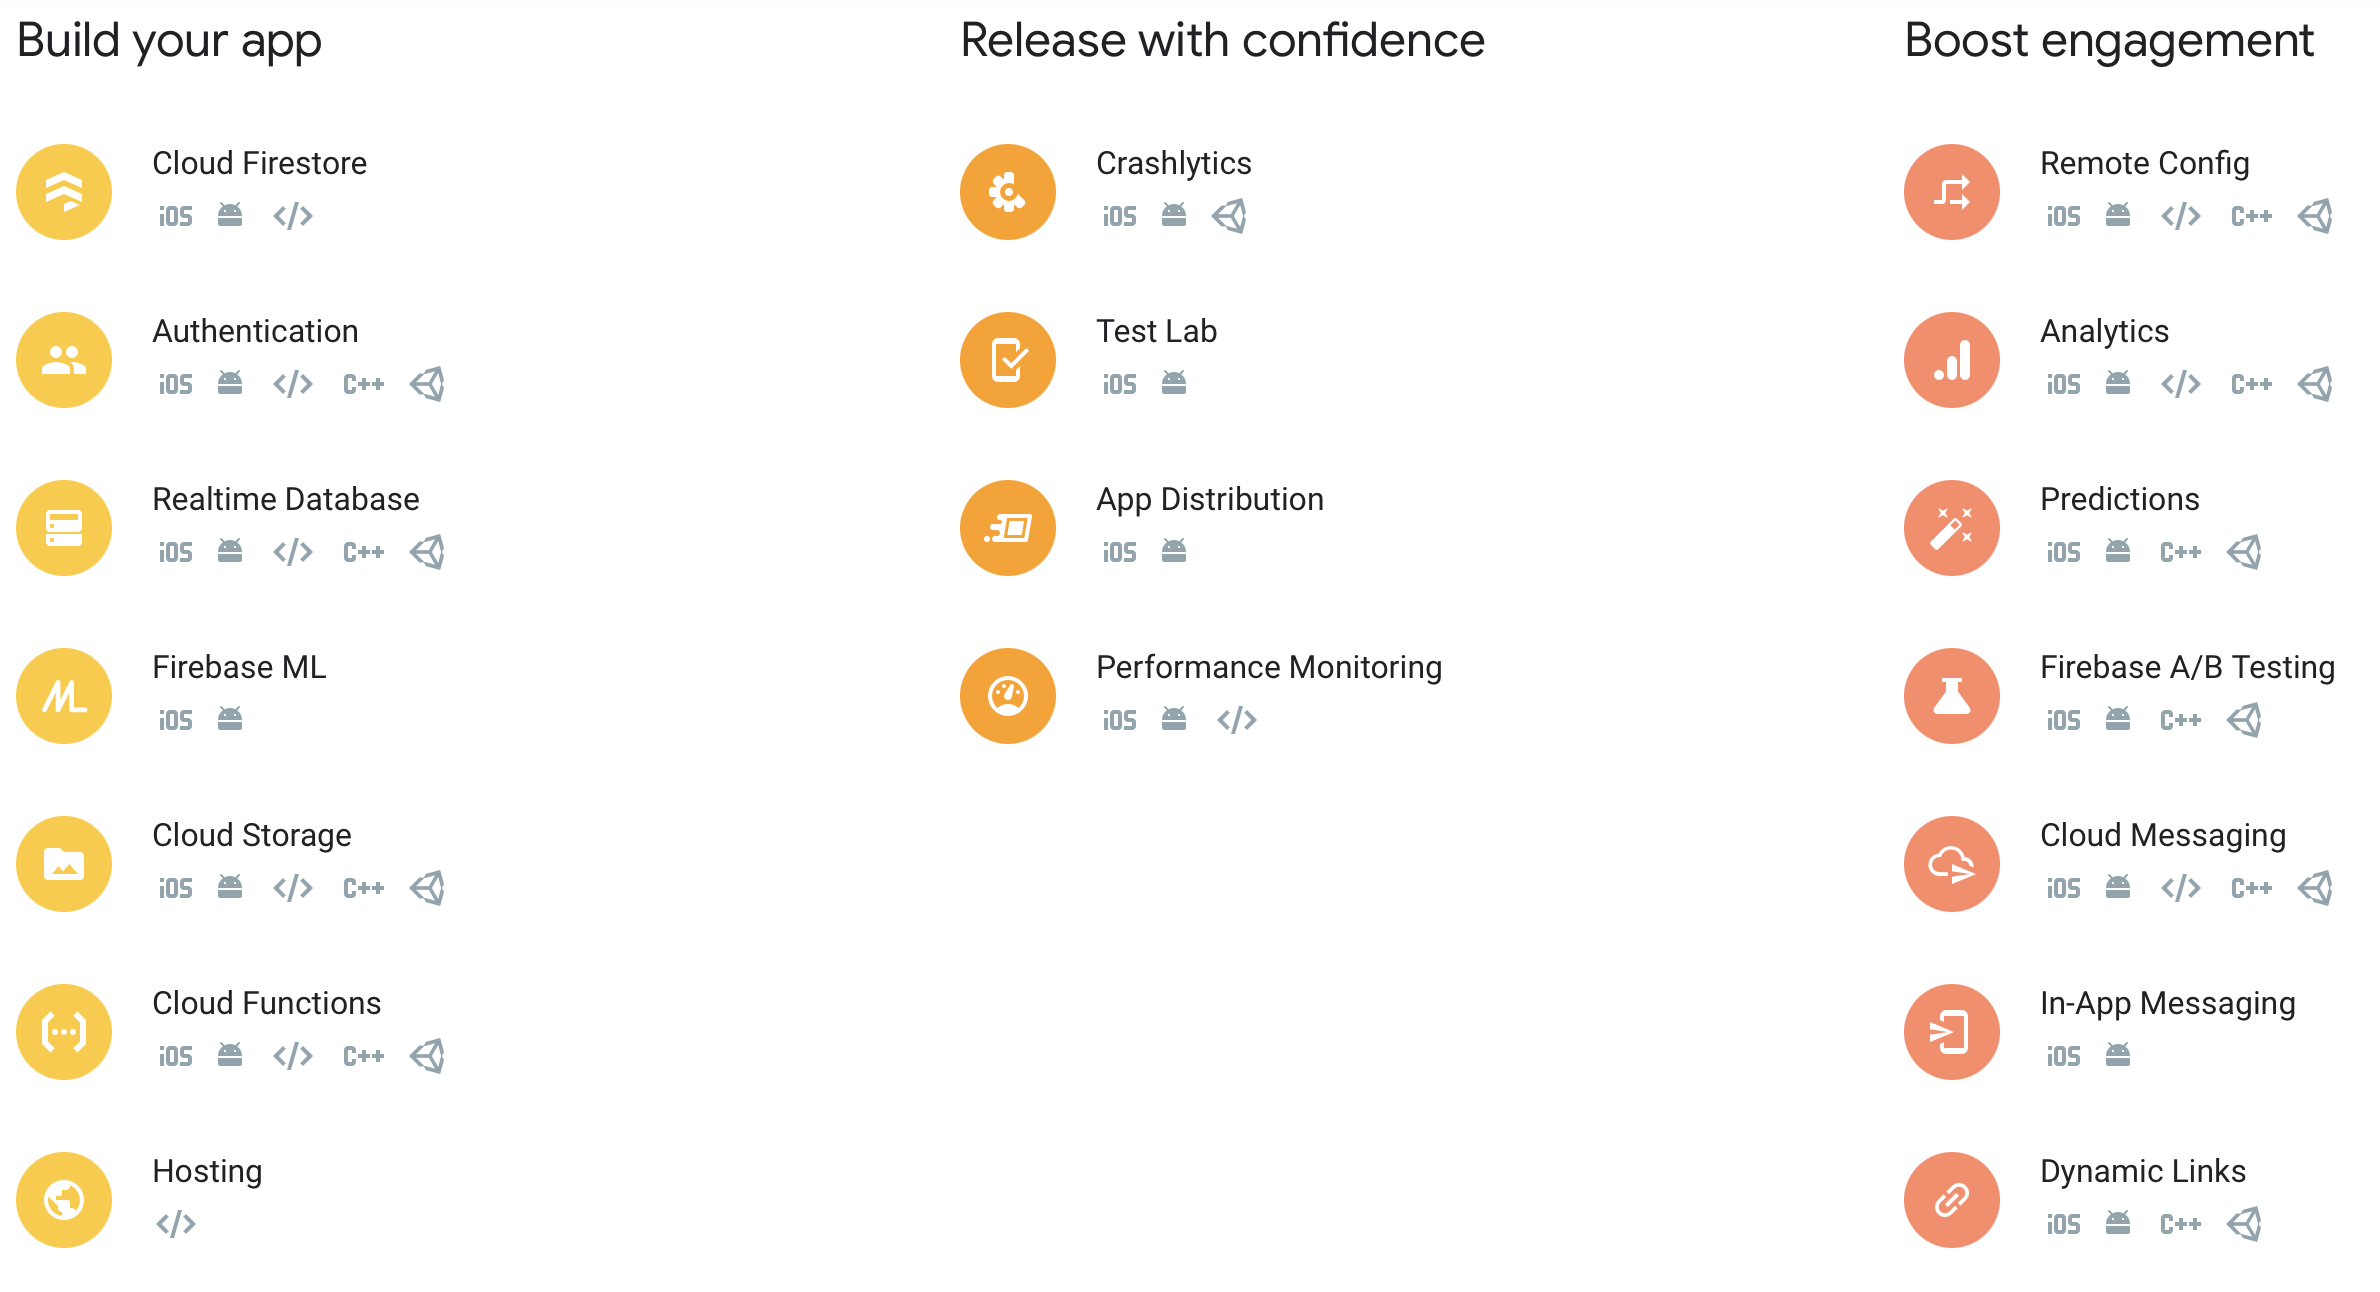
\includegraphics[scale=0.3]{images/firebase_offerings.png}
    \end{center}
    \caption{Firebase product offerings}
    \label{firebase_compute_offerings}
\end{figure}

However, all these benefits come at the cost: Firebase is closed-source and has vendor lock-in built into its design. Firebase is much more opinionated than the other back-end solutions that we have explored, in the following ways:

\begin{itemize}
    \item Databases are accessed directly by clients instead of a back-end endpoint through the Firestore or Realtime Database APIs
    \item Firebase-provided databases are strictly non-relational.
    \item On-demand compute comes in the form of Firebase Cloud Functions, which is designed for small bursts of computation instead of long-running loops. The latter is still possible, but the resulting bill would be unfeasible.
    \item Cloud Functions currently only supports REST APIs and only supports a limited range of runtime environments \cite{TODO}.
\end{itemize}

Despite these, Firebase provides key functionality which may prove extremely valuable in continuing development for this project. Even if not implemented in this run of the project, Firebase offers out-of-the-box solutions for file storage, app crash analytics, search engine optimisation, A/B testing and even (limited) machine learning tasks. Therefore, it is undisputably the platform that will enable the fastest development of a workable product.

In summary, the features that it provides will service the needs of future development on this project for a long time to come. Even if it should scale beyond that point, there should be enough resources to facilitate a migration away from Firebase anyway.
